\documentclass[UTF8]{ctexart}
\usepackage{subfigure}
\usepackage{caption}
\usepackage{amsmath,bm}
\usepackage{amssymb}
\usepackage{pifont}
\usepackage{geometry}
\usepackage{graphicx}
\usepackage{gensymb}
\usepackage{wrapfig}
\usepackage{titlesec}
\usepackage{float}
\usepackage{diagbox}
\usepackage{fancyhdr}
\usepackage{color}
\usepackage{bm}
\usepackage{siunitx}
\usepackage{ulem}
\usepackage{CJKulem}
\pagestyle{plain}
\geometry{a4paper,scale=0.8}
\CTEXsetup[format+={\raggedright}]{section} 
\title{现代计算机体系架构2022期末}
\author{Deschain}
\titlespacing*{\section}
{0pt}{0pt}{0pt}
\titlespacing*{\subsection}
{0pt}{0pt}{0pt}
\titlespacing*{\paragraph}
{0pt}{0pt}{0pt}
\titlespacing*{\subparagraph}
{0pt}{0pt}{0pt}
\titleformat*{\section}{\normalsize}
\titleformat*{\subsection}{\normalsize}
\begin{document}
\maketitle
\section*{一、Mutiple Choice(one answer)(30pts)}
\subsection*{1. In following discussion of reducing execution time T, which one is \textit{\bfseries always correct}? Assume everything else is kept unchanged.}
(a) T is reduced if we increase the number of pipeline stages\\
(b) T is reduced if we increase the number of processing cores\\
(c) T is reduced if we increase the working frequency of cores\\
(d) T is reduced if we increase the capacity of main memory\\

\subsection*{2. In the following discussion of evaluating a computer system, which one is correct?}
(a) Performance is one important metric\\
(b) Power consumption is one important metric\\
(c) Reliability is one important metric\\
(d) All of above\\

\subsection*{3. Please select the correct die yield, assuming a wafer yield of 1, die area of 2$cm^2$, defect density of 0.025 per $cm^2$, and N = 13.5.}
(a)0.42\\
(b)0.52\\
(c)0.32\\
(d)0.62\\

\subsection*{4. In the following scenarios of memory accessing, which one is {\bfseries\textit {impossible}}?}
(a) TLB hit, cache hit, page hit;\\
(b) TLB miss, cache hit, page hit;\\
(c) TLB hit, cache hit, page miss;\\
(d) TLB hit, cache miss, page hit;\\

\subsection*{5. To support register renaming, each register in Register File(RF) has two 3-bit counters: NI and LI. Assume that the current state in RF is 
NI(\$1)=3, LI(\$1)=4, NI(\$2)=2, LI(\$2)=1. Now a new instruction {\bfseries\textit{ADDI \$1, \$2, 2}} is dispatched to RUU. What are the values in RF counters?}
(a) NI(\$1)=4, LI(\$1)=5, NI(\$2)=3, LI(\$2)=2\\
(b) NI(\$1)=3, LI(\$1)=4, NI(\$2)=2, LI(\$2)=1\\
(c) NI(\$1)=4, LI(\$1)=5, NI(\$2)=2, LI(\$2)=1\\
(d) NI(\$1)=3, LI(\$1)=4, NI(\$2)=3, LI(\$2)=2\\

\subsection*{6. Which of the following computing schemas does NOT belong to computing-in-memory (CIM)?}
(a) Current-manner computing\\
(b) Charge-manner computing\\
(c) Systolic-manner computing\\
(d) Digital-manner computing\\

\subsection*{7. In following discussion about handling of I/O requests with "interrupt" and "polling" methods, which one is correct?}
(a)"Interrupt" is always faster than "polling"\\
(b)"Interrupt" is always slower than "polling"\\
(c)"interrupt" is as fast as "polling"\\
(d) None of above is correct\\ 

\subsection*{8. In following discussion about pipeline design, which one is {\bfseries\textit{incorrect}}?}
If we increase pipeline stage number,\\
(a) ILP can be increased\\
(b) Instruction execution time can be increased\\
(c) Throughput can be increased\\
(d) Data hazards can be increased\\

\subsection*{9. In the following discussion about cache {\bfseries\textit{miss rate}}, which one is correct? Assume that other design factors are kept unchanged.}
(a) Miss rate is always decreased if we increase cache set number\\
(b) Miss rate is always decreased if we increase associativity\\
(c) Miss rate is always decreased if we increase cache block size\\
(d) None of above\\

\subsection*{10. In following comparison between CISC and RISC, which one is incorrect?}
(a) Using RISC normally generates more instruction numbers\\
(b) Using RISC normally requires less design complexity\\
(c) Using RISC normally generates less memory accesses\\
(d) Using RISC normally achieves higher clock frequency\\

\subsection*{11. Which one of following data dependencies does not exist?}
(a) Read before Read dependency\\
(b) Read before Write dependency\\
(c) Write before Read dependency\\
(d) Write before Write dependency\\

\subsection*{12. What type of locality does a one-word set associativity cache take advantage?}
(a) Spacial locality\\
(b) Temporal locality\\
(c) Both of them\\
(d) None of them\\

\subsection*{13. Which of following will NOT limit maximum BUS throughput?}
(a) Device number connected to the BUS\\
(b) Total length of the BUS\\
(c) Arbitration method of the BUS\\
(d) None of them\\

\subsection*{14. Which bandwidth is {\bfseries low} for weight-stationary(input-parallel), input-stationary(weight-parallel), and output-stationary optimization in CNN processor?}
(a) Weight bandwidth, Input bandwidth, Output bandwidth\\
(b) Input bandwidth, Weight bandwidth, Output bandwidth\\
(c) Output bandwidth, Output bandwidth, Input bandwidth and weight bandwidth\\
(d) None of them\\

\subsection*{15. Which of the following techniques can NOT improve the energy efficiency of a netural network processor?}
(a) Allocate local storage near the computing unit\\
(b) Use higher precision activations and weights\\
(c) Exploit the sparsity of netual networks\\
(d) Use computing-in-memory technique\\

\section*{二、Scalar MIPS Processor. (10pts)}
1. Compare the performance of three different MIPS implementations - a single cycle machine with a 10 ns (nanosecond) clock, a multi-cycle machine with a 2 ns 
clock, and a five stage scalar pipelined machine with a 2 ns clock. For both multi-cycle and pipelined designs, the execution is partitioned into 5 stages: \textit{Fetch, 
Decode, Execution, Memory, and WriteBack}. In the case of the pipelined machines, assume the pipeline is initially empty. (Assume no cache miss)\\
For following instructions, please calculate total execution time.\\
add \$2, \$1, \$3\\
add \$1, \$2, \$3\\
store \$1, 5(\$8)\\
load \$1, 2(\$2)\\
add \$2, \$3, \$4\\
i. -total time for the single cycle machine to complete\\
ii. -total time for the multi-cycle machine to complete\\
iii. -total time for pipelined machine without data forwarding to complete\\
iv. -total time for pipelined machine with data forwarding to complete\\

\section*{三、Superscalar MIPS Processor. (10pts)}
The following figure shows the RUU unit (4-entry RUU), with 2 instructions in the RUU. Please fill in (NI:LI) for \$1 and \$2. (4pts)\\
\begin{figure}[H]                                             
    \centering                                                
    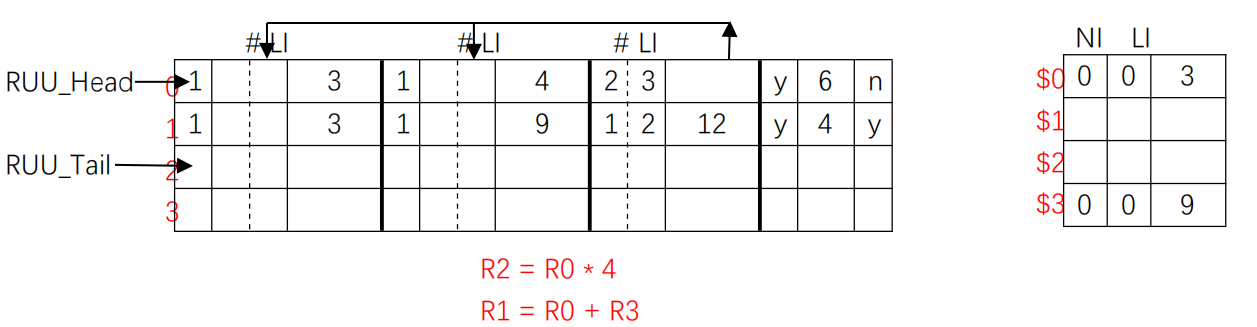
\includegraphics[width=14cm,height=4cm]{3-1.png}        
    \caption*{}                                                                              
\end{figure}  
A new instruction: \underline{\bfseries R2=R2+R1} is added to the RUU, please fill in all changes (assume that RUU entry doesn't finish execution yet)(6pts)\\
\begin{figure}[H]                                            
    \centering                                                
    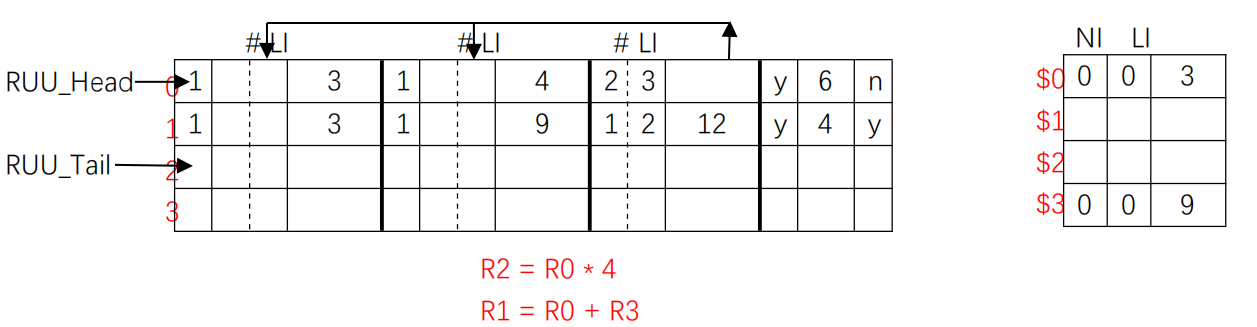
\includegraphics[width=14cm,height=4cm]{3-1.png}        
    \caption*{}                                                                                 
\end{figure}  

\section*{四、Memory System. (10pts)}
Assume there is a simple DRAM array shown in the following figure, which is composed of eight rows and eight columns. Each crossing of one row and one column
stores one bit of data. Thus, there are 64 bits data in total. The data address is represented with 6-bit, first three of which are used as row address bits and 
last three are used for column addressing. For example, the data at crossing of row-0 and column-0 (highlighted with) is addressed as 000000.\\
\begin{figure}[H]                                            
    \centering                                                
    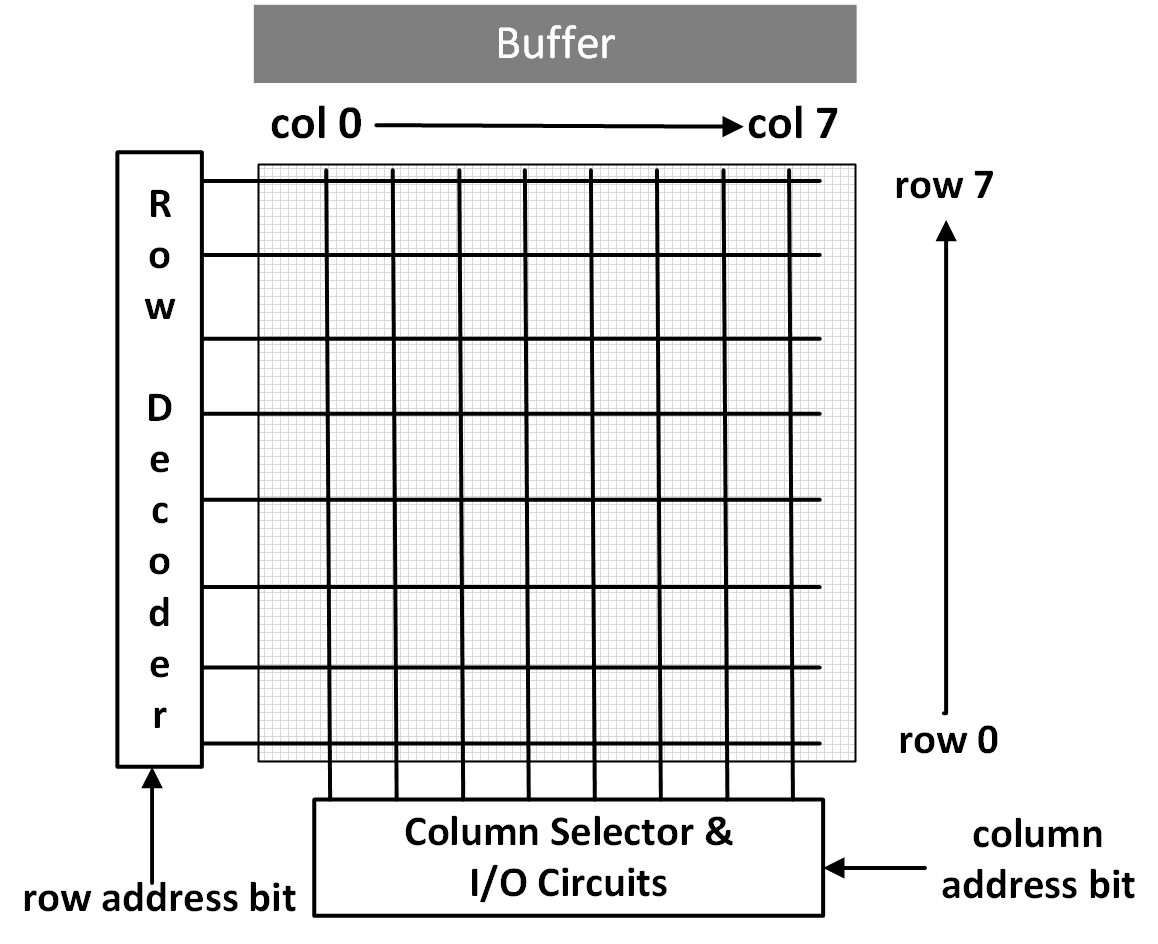
\includegraphics[width=7cm,height=6cm]{4-1.png}        
    \caption*{}                                                                                 
\end{figure}  
Each request only accesses {\bfseries one bit of data}. The access flow is as follows:\\
(1) If data is not in the buffer, load all the row containing data into the buffer.\\
(2) Access the data according to column address.\\
Assume the time to load a row to the buffer is 10 cycles. And it takes 1 cycle to access data if it is already in the buffer. Buffer is empty at the beginning.\\
i. Please calculate the time to access 1-bit data with following addresses\\
000101 001100 000101 001101 100100\\
ii. If the accessing sequence can be adjusted, what is the minimum access time?\\
iii. Can you change the address format to achieve the lower bound of access time? Just identify which bits are used for row addressing.\\

\section*{五、Cache Architecture. (15pts)}
1. If the processor with IL1 and DL1 has a CPI-ideal of 1.25, a 100 cycle miss penalty, 40\% load/store instructions, a 2\% I\$ miss rate, and a 5\% D\$ miss rate,
what is the CPI-stall with memory stalls taken into account? (5 pts)\\
2. In order to reduce CPI, we add one uniform L2. Its hit latency is 5 cycle. And its miss rate is 0.2\%. Please recalculate CPI-stall. (5 pts)\\
3. Consider a four word cache memory (initially empty), a sixteen word main memory, and the following string of address references (given as word addresses). The 
following questions are based on this.\\\
\centerline{\bfseries 2 3 9 10 2 10 2 3}\\
Show the state of the cache after tha last reference if the cache is two-way set associative with two word blocks and FIFO replacement.(4 pts)
\begin{figure}[H]                                            
    \centering                                                
    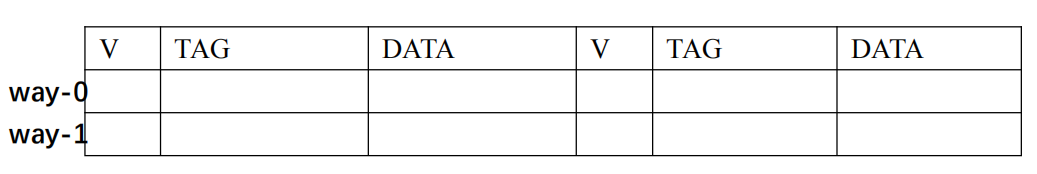
\includegraphics[width=10cm,height=2cm]{5.png}        
    \caption*{}                                                                                 
\end{figure}  
How many misses are there in total? (1 pt)\\
\centerline{(a)4 (b)5 (c)6 (d)7 (e)8}\\

\section*{六、Disk+I/O Systems Design. (10 pts)}
Consider a disk workload of 32KB reads and writes where the user program executes 200,000 instructions between disk I/O operation, a processor
that executes 1 billon instructions/second and that averages 50,000 OS instructions to process a disk I/O operation, a memory-I/O bus that sustains
a transfer rate of 1000MB/second. disk controllers with a DMA transfer rate of 320MB/second that can accommodate up to 4 disks per controller, and 
disk drives with a transfer rate of 100MB/second and an average seek plus rotational latency plus controller overhead of 6ms (all of the sectors in 
a disk read/write are located consecutively on the disk).\\
1. Which is the bottleneck, the processor or the memory-I/O bus?(3 pts)\\
2. What is the maximum sustainable I/O rate?(3 pts)\\
3. How many disks and disk controllers are needed to achieve that rate?(4 pts)\\

\section*{七、Multiple Processors. (5 pts)}
Assume there is a two-processor computer, shown as follows. There is one thread running on each core, and these two threads share a data A, which is located
at main memory at the beginning. For each processor, the access flow to data is listed as follows.\\
1. For read access, if data is in its own cache, read data directly. Otherwise, send read reuqest to the bus, and store data in the cache agter receiving data 
from the bus.\\
2. For write request, if data is in its own cache, update data. Then, send updated data to the bus. If data is not in the cache, send read request to the bus, 
and store data in the cache after receiving data from the bus. At last, updata data and send updated data to the bus.\\
3. When a cache sees a read request on the bus, if it has the data required, send data on the bus. When a cache sees an updated data on the bus, if it has the 
data required, send data on the bus. When a cache sees an updated data on the bus, if it has the data required, updata its data.\\
4. If memory sees a read request on the bus, it will send data on the bus if no other cache response. If memory sees an updated data on the bus, it will update 
its data.\\
\begin{figure}[H]                                            
    \centering                                                
    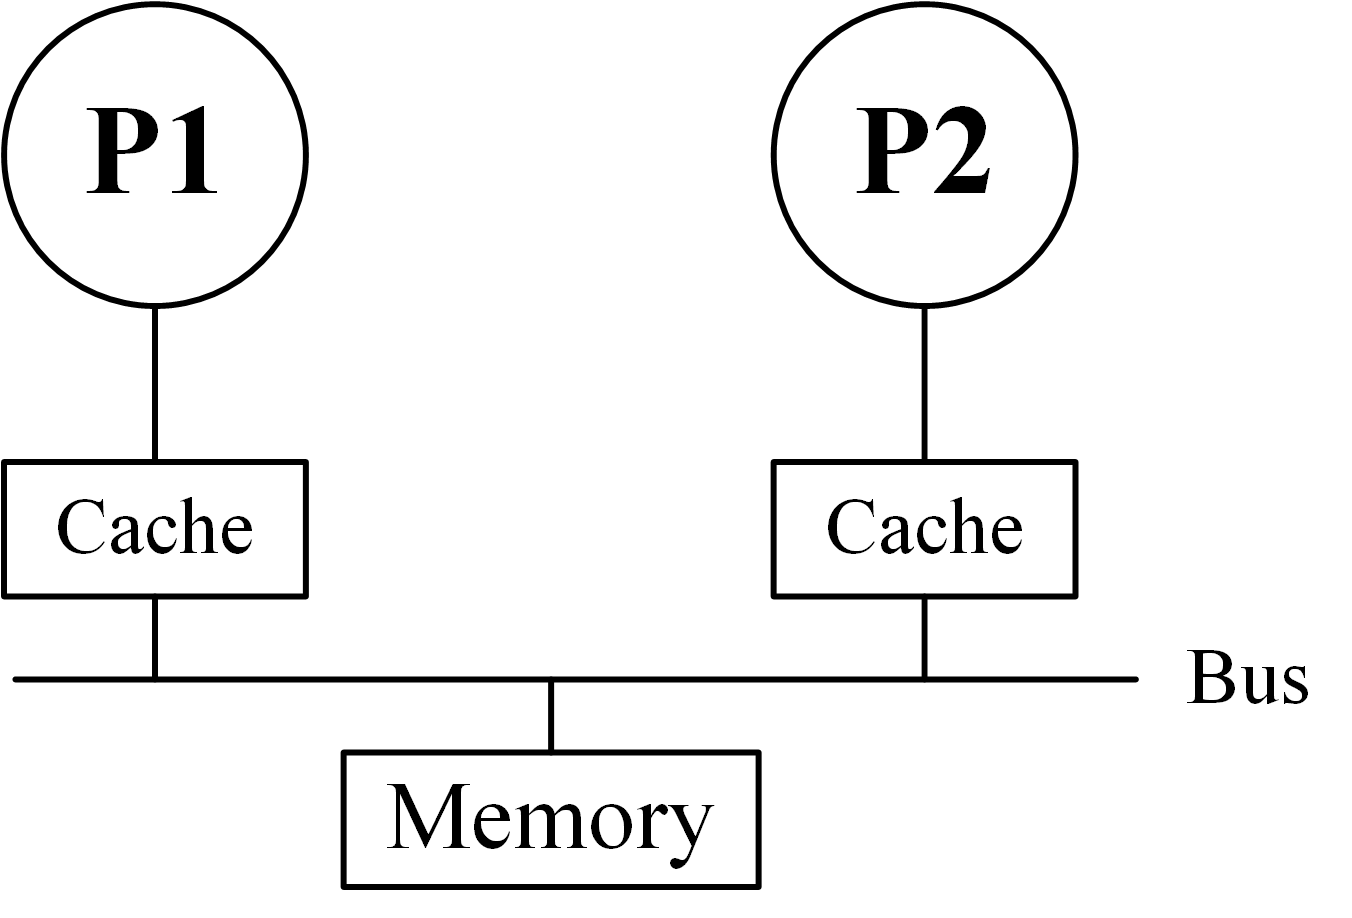
\includegraphics[width=6cm,height=4cm]{7.png}        
    \caption*{}                                                                                 
\end{figure}  
These two threads perform four following access requests to the data A\\
T-1: Read A\quad\quad T-1: Write A=2\quad\quad T-2: Write A=3\quad\quad T-1: Read A\\
1. Please identify values of A in each cache after the four requests.\\
P1-Cache=\quad\quad P2-Cache=\quad\quad Memory=\quad\quad\\
2. How many read requests and data signals are transferred on the bus?\\
No.of read requests:\quad\quad No.of data signals:\\

\section*{八、Warehouse-scale computer. (12 pts)}
MapReduce enables large amounts of parallelism; however, there are limits to the level of parallelism. For example, for redundancy, MapReduce will 
read data blocks from multiple nodes, consuming disk and potentially network bandwidth. Assume a total dataset size of 400 GB, a 10 sec/GB map rate, 
and a 20 sec/GB reduce rate. Also assume that 30\% of the data must be read from remote nodes, and the dataset is broken up into equal size of files 
among the nodes. Local disk bandwidth is 200MB/s; disk bandwidth between nodes in the same rack is 100MB/s; and disk bandwidth betwen nodes in 
different racks is 10MB/s.\\
a. Assume that all nodes are in the same rack. What is the expected runtime with 5 nodes? 1000 nodes? Are the bottlenecks different at these node 
sizes? (4pts)\\
b. Assume that there are 40 nodes per pack and that any remote read/write has an equal chance of going to any node. What is the expected runtime at 
80 nodes? 800 nodes? Discuss the bottleneck at these node sizes. (4 pts)\\
c. An important consideration is minimizing data movement as much as possible. Assume that there are 40 nodes per rack, and 800 nodes are used in the 
MapReduce job. What is the runtime if remote accesses are within the same rack 20\% 0f the time? 80\% of the time? Discuss the bottleneck at these 
node sizes. (4 pts)\\

\section*{九、GPU. (15 pts)}
a. Explain the meaning of SP, SM, Warp, Thread group and Grid in a GPU. Draw a picture to show the basic architecture of GPU.(3pts)\\
b. When we execute a program on a GPU, each computation for a Warp needs 10 cycles and each memory access is 300 cycles (without cache miss) or 3000 
cycles (with cache miss). Please calculate the bumber of warp in a SM to avoid the computing unit waiting for memory access for the best case or the 
worst case.(4 pts)\\
c. Describe the working flow for a CPU to call a GPU to execute a task. (3 pts) \\
d. Assume a GPU architecture that contains {\bfseries 10 SIMD processors}. Each SIMD instruction has a width of 32 and each SIMD processor contains 8 
lanes for single-precision arithmatic and other instructions, meaning that each non-diverged SIMD instruction can produce {\bfseries 32 results every 
4 cycles}. Assume a kernel that has divergent branches that causes on average {\bfseries 80\% of the threads to be active. 70\% of all SIMD instructions} 
executed are single-precision arithmatic. Assume an average SIMD {\bfseries instruction issue rate of 0.85}. The clock speed of the GPU is {\bfseries 1.5 
GHz}. (5 pts)\\
\begin{itemize}
    \item[]
    i. Compute the throughput, in GFLOP/sec, for this kernel on this GPU.\\
    ii. Assume that you have the following choices:
    \begin{itemize}
        \item[]
        (1) Increasing the number of single-precision lanes to 16\\
        (2) Increasing the number of SIMD processors to 15 (assume this change doesn't affect any other performance metrics and that code scales 
to the additional processors)\\
        (3) Adding a cache that will effectively increase instruction issue rate to 0.95. \\
        What is speedup in throughput for each of these improvements?\\
    \end{itemize}
\end{itemize}
    


\newpage
\section*{一、Mutiple Choice(one answer)(30pts)}
1.C\quad 2.D\quad 3.C\quad 4.C\quad 5.C\quad 6.C\quad 7.D\quad 8.A\quad 9.B\quad 10.C\quad 11.A\quad 12.B\quad 13.D\quad 14.A\quad 15.B\quad

\section*{二、Scalar MIPS Processor. (10pts)}
i.\quad 50ns\\
ii.\quad 42ns\\
iii.\quad (如果寄存器堆是先写后读的) 26ns (如果不是)30ns\\
iv.\quad 18ns

\section*{三、Superscalar MIPS Processor. (10pts)}
1.
\begin{figure}[H]                                            
    \centering                                                
    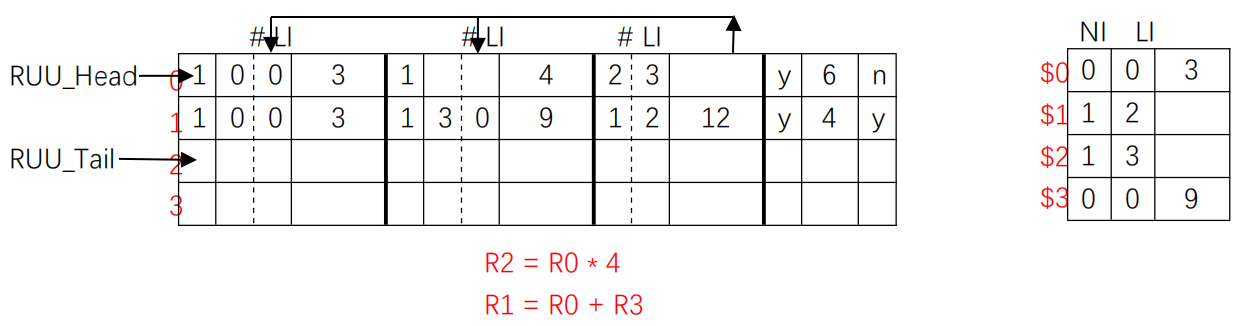
\includegraphics[width=14cm,height=4cm]{3-1-ans.png}        
    \caption*{}                                                                                 
\end{figure}  
2.
\begin{figure}[H]                                            
    \centering                                                
    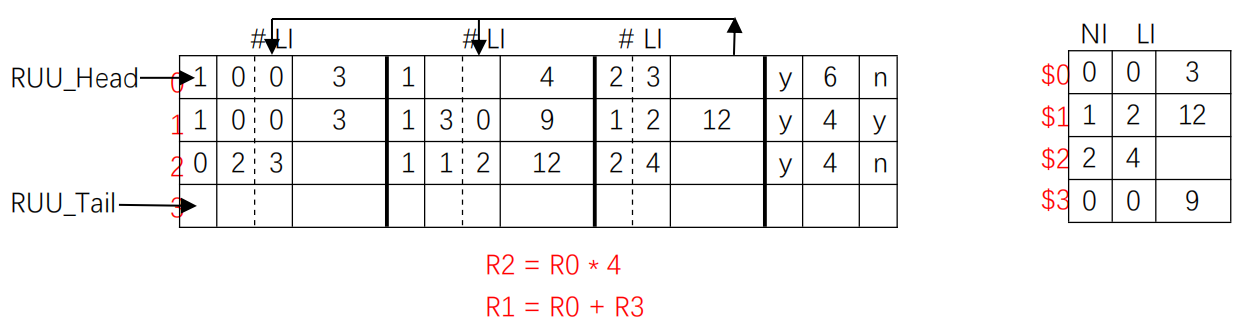
\includegraphics[width=14cm,height=4cm]{3-2-ans.png}        
    \caption*{}                                                                                 
\end{figure}  

\section*{四、Memory System. (10pts)}
i. 55cycles\\
ii. 000101 000101 001100 001101 100100, 35cycles\\
iii. 观察地址序列,可以看出第一位一直是0,第四位一直是1,第五位一直是0。如果用一、四、五位作为行地址,则访问时间最短,为15 cycles。\\

\section*{五、Cache Architecture. (15pts)}
1. $1.25+2\%\times1.25\times100+5\%\times40\%\times1.25\times100=6.25$\\
2.一条指令引发L1 cache缺失的概率是$2\%+5\%\times40\%=4\%$。题中说L2 cache的缺失率是$0.2\%$,但没有说是局部缺失率还是全局缺失率。根据常识,L2 cache的局部缺失率
是很高的,所以这里的$0.2\%$应该是全局缺失率。\\
$CPI-stall=1.25+4\%\times1.25\times5+0.2\%\times1.25\times100=1.75$\\
3.(1)
\begin{figure}[H]                                            
    \centering                                                
    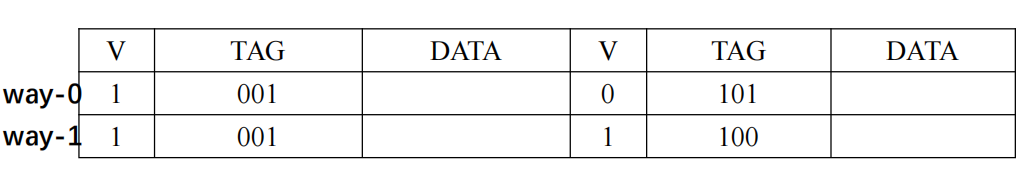
\includegraphics[width=10cm,height=2cm]{5-3.png}        
    \caption*{}                                                                                 
\end{figure}  
(2) a
\section*{六、Disk+I/O Systems Design. (10 pts)}
1. 处理器每秒执行$10^9$条指令,每次I/O操作需要$50000$条指令,即处理器每秒能执行$10^9\div50000=20000$次I/O操作。
总线的每秒传输$320MB$的数据,每次I/O操作传输$32KB$的数据,即总线每秒能执行$1000\times1024\div32=32000$次I/O操作。
因此,处理器是这个架构的瓶颈。\\
2.根据1中的分析,最大的I/O率为处理器支持的I/O率,即$20000/s$。\\
3.每秒$20000$次I/O,需要的数据传输率为$32KB\times20000=625MB/s$。
一次硬盘读写操作中,硬盘驱动先用$6ms$找到数据,然后用$100MB/s$的速度传输一个$32KB$的数据块。也就是说,传输$32KB$的数据块用时
$0.006+32\div(100\times1024)=0.0063125s=6.3125ms$,数据率为$32\div0.0063125=4.95MB/s$。
为了达到$625MB/s$的数据率,需要$625/div4.95=126.3=126$块硬盘。
一块硬盘控制器能控制4块硬盘,126块硬盘应该配置32块硬盘控制器。4块硬盘的数据率为$4.95MB/s\times4=19.8MB/s$,小于硬盘控制器的
数据传输率$320MS/s$,所以这个方案是可行的。
\section*{七、Multiple Processors. (5 pts)}
1. 3 3 3\\
2.分析流程:
(1) T-1 Read A: T-1发起一次read request, Memory通过总线传输一次数据。\\
(2) T-1 Write A=2: T-1通过总线传输更新后的数据,Memory更新数据。\\
(3) T-2 Write A=3: T-2发起一次read request,T-1通过总线传输数据。T-2通过总线传输更新后的数据,T-1和Memory更新数据。\\
(4) T-1 Read A: 直接读取,不需要利用总线。\\
共计2个读请求,4次数据传输。\\
\section*{八、Warehouse-scale computer. (12 pts)}
a. \\
5个节点,每个有$80GB$数据。其中$70\%\times80GB=56GB$数据在本地,读入速度为$200MB/s$,读入用时$56GB\div200MB/s=286.72s$。
$30\%\times80GB=24GB$的数据在其他节点上,读入速度为$100MB/s$,读入用时$24GB\div100MB/s=245.76s$。
读取数据总用时为$286.72+245.76=532.48s$。
map操作用时为$10s/GB\times80GB=800s$,reduce操作用时为$20s/GB\times80GB=1600s$。
总用时$532.48+800+1600=2932.48s$。\\

1000个节点,每个有$0.4GB=409.6MB$数据。
其中$70\%\times409.6MB=286.72MB$数据在本地,读入速度为$200MB/s$,读入用时$286.72MB\div200MB/s=1.4336s$。
$30\%\times409.6MB=122.88MB$的数据在其他节点上,读入速度为$100MB/s$,读入用时$122.88MB\div100MB/s=1.2288s$。
读取数据总用时为$1.4336+1.2288=2.6624s$。
map操作用时为$10s/GB\times0.4GB=4s$,reduce操作用时为$20s/GB\times0.4GB=8s$。
总用时$2.6624+4+8=14.6624s$。\\

瓶颈都是map和reduce的用时。\\
b. \\
80个节点,每个有$5GB$数据,共有2个rack。
其中$70\%\times5GB=3.5GB$数据在本地,读入速度为$200MB/s$,读入用时$3.5GB\div200MB/s=17.92s$。
$50\%\times30\%\times5GB=0.75GB=768MB$的数据在同一rack中的其他节点上,读入速度为$100MB/s$,读入用时$768MB\div100MB/s=7.68s$。
$50\%\times30\%\times5GB=0.75GB=768MB$的数据在另一rack中,读入速度为$10MB/s$,读入用时$768MB\div10MB/s=76.8s$。
读取数据总用时为$17.92+7.68+76.8=102.4s$。
map操作用时为$10s/GB\times5GB=50s$,reduce操作用时为$20s/GB\times5GB=100s$。
总用时$102.4+50+100=252.4s$。\\

800个节点,每个有$0.5GB$数据,共有20个rack。
其中$70\%\times0.5GB=0.35GB$数据在本地,读入速度为$200MB/s$,读入用时$0.35GB\div200MB/s=1.792s$。
$5\%\times30\%\times0.5GB=0.0075GB=7.68MB$的数据在同一rack中的其他节点上,读入速度为$100MB/s$,读入用时$7.68MB\div100MB/s=0.0768s$。
$95\%\times30\%\times0.5GB=0.1425GB=145.92MB$的数据在另一rack中,读入速度为$10MB/s$,读入用时$145.92MB\div10MB/s=14.592s$。
读取数据总用时为$1.792+0.0768+14.592=16.4608s$。
map操作用时为$10s/GB\times0.5GB=5s$,reduce操作用时为$20s/GB\times0.5GB=10s$。
总用时$16.7648+5+10=31.7648s$。\\

瓶颈为读取数据的用时。\\

c.\\
800个节点,每个有$0.5GB$数据,共有20个rack。
其中$70\%\times0.5GB=0.35GB$数据在本地,读入速度为$200MB/s$,读入用时$0.35GB\div200MB/s=1.792s$。
$20\%\times30\%\times0.5GB=0.03GB=30.72MB$的数据在同一rack中的其他节点上,读入速度为$100MB/s$,读入用时$30.72MB\div100MB/s=0.3072s$。
$80\%\times30\%\times0.5GB=0.12GB=122.88MB$的数据在另一rack中,读入速度为$10MB/s$,读入用时$122.88MB\div10MB/s=12.288s$。
读取数据总用时为$0.3072+12.288=12.5952s$。
map操作用时为$10s/GB\times0.5GB=5s$,reduce操作用时为$20s/GB\times0.5GB=10s$。
总用时$12.5952+5+10=27.5952s$。\\
瓶颈为读取数据的用时。\\

800个节点,每个有$0.5GB$数据,共有20个rack。
其中$70\%\times0.5GB=0.35GB$数据在本地,读入速度为$200MB/s$,读入用时$0.35GB\div200MB/s=1.792s$。
$80\%\times30\%\times0.5GB=0.12GB=122.88MB$的数据在同一rack中的其他节点上,读入速度为$100MB/s$,读入用时$122.88MB\div100MB/s=1.2288s$。
$20\%\times30\%\times0.5GB=0.03GB=30.72MB$的数据在另一rack中,读入速度为$10MB/s$,读入用时$122.88MB\div10MB/s=3.072s$。
读取数据总用时为$1.2288+3.072=4.3008s$。
map操作用时为$10s/GB\times0.5GB=5s$,reduce操作用时为$20s/GB\times0.5GB=10s$。
总用时$4.3008+5+10=19.3008s$。\\
瓶颈为map和reduce的用时。\\
\section*{九、GPU. (15 pts)}
a.\\
SP: streaming processor\\
SM: streamming multiprocessor\\
Warp: smallest thread scheduling unit. In NVIDIA GPUs, a warp is 32 threads.\\
Thread group: (没找到定义,但我猜这个是"thread block")a group of warps\\
Grid: a collection of blocks \\
\begin{figure}[H]                                            
    \centering                                                
    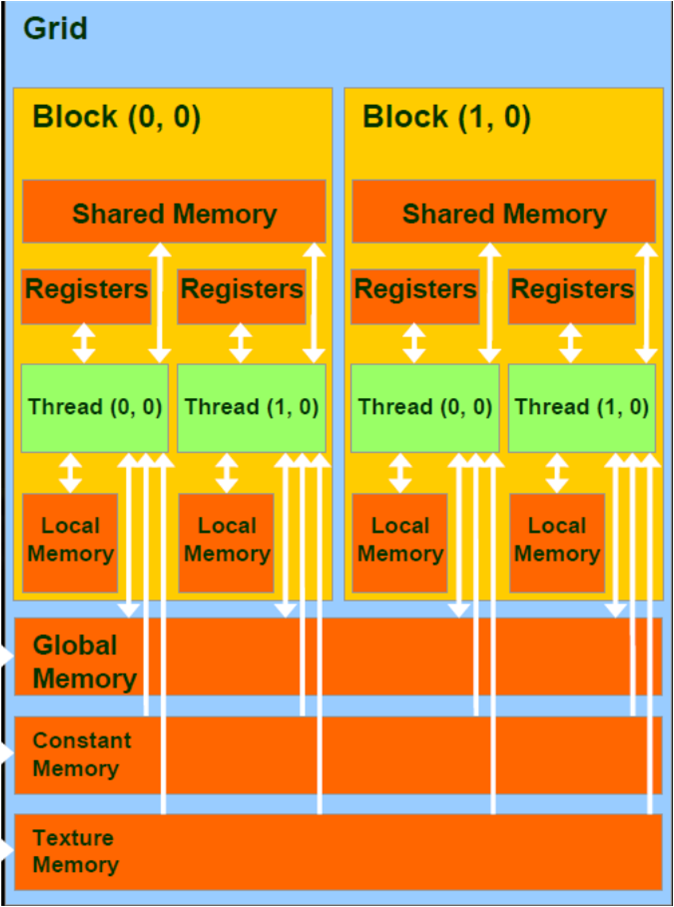
\includegraphics[width=5cm,height=8cm]{9.png}        
    \caption*{}                                                                                 
\end{figure}  
b. 30 for best case, 300 for worst case\\
c.\\
\begin{enumerate}
    \item Copy input data from CPU memory to GPU memory 
    \item Laod GPU code and execute item 
    \item Copy results from GPU memory to CPU memory
\end{enumerate}
d.\\
i. $0.85\times10\times80\%\times8\times70\%\times1.5G=57.12GFLOP/sec$\\
ii. \\
(1)$0.85\times10\times80\%\times16\times70\%\times1.5G=114.24GFLOP/sec$\\
(2)$0.85\times15\times80\%\times8\times70\%\times1.5G=85.68GFLOP/sec$\\
(3)$0.95\times10\times80\%\times8\times70\%\times1.5G=63.84GFLOP/sec$\\

\end{document}